\documentclass[11pt]{report}

\usepackage[portuguese]{babel}
\usepackage[utf8]{inputenc}
\usepackage{graphicx}
\usepackage{hyperref}
\usepackage{indentfirst}
\usepackage{kantlipsum}
\usepackage{float}
\usepackage{listings}
\usepackage{mathtools}
\usepackage{amsmath}
\usepackage{url}
\usepackage[margin=0.8in]{geometry}
\usepackage{biblatex}
\usepackage{multirow}
\usepackage{fancyhdr}
\usepackage[table,xcdraw]{xcolor}
\bibliography{biblio.bib}

\lstset{language=Prolog}

\hypersetup{
    colorlinks=true,
    linkcolor=black,
    citecolor=black,
    filecolor=black,
    urlcolor=black
}

\newlength{\normalparindent}
\setlength{\normalparindent}{\parindent}
\setlength{\parindent}{\normalparindent}

\newcommand{\blank}[1]{\hspace*{#1}}

\renewcommand{\headrulewidth}{0pt}

\pagestyle{fancy}
\fancyhf{}
\rhead{
\includegraphics [scale=0.5]{uproject_new_2.png}}
\rfoot{\thepage}

\begin{document}

\thispagestyle{empty}

\begin{center}
	
	
\includegraphics [scale=0.5]{uplogo500.png}
	\linebreak \linebreak \linebreak \linebreak \linebreak
	\linebreak \linebreak \linebreak \linebreak \linebreak
	\begin{Huge}
		\textbf{U.Project Website} \linebreak \linebreak
	\end{Huge}
	\begin{Large}
		\textbf{Relatório de Estágio} \linebreak \linebreak
	\end{Large}
	\linebreak
	\linebreak
	\linebreak
	\linebreak
	\linebreak
	\linebreak
	Orientadores:
	\linebreak
	\linebreak
	Bruno Fernando Reis Ribeiro Silva - \href{mailto: brunosilva@uproject.pt}{\texttt{brunosilva@uproject.pt}}
	\linebreak
	Márcio Filipe Vilela Fontes - \href{mailto: marciofontes@uproject.pt}{\texttt{marciofontes@uproject.pt}}
	\linebreak
	\linebreak
	\linebreak
	\linebreak
	UPTEC - Parque de Ciência e Tecnologia da Universidade do Porto
	\linebreak
	Rua Alfredo Allen, nº455/461, 4200-135 - Porto, Portugal
	\linebreak
	\linebreak
	\linebreak
	\linebreak
	5 de Setembro de 2015
\end{center}

\newpage

\pagenumbering{roman}

\chapter*{Agradecimentos}
\addcontentsline{toc}{chapter}{Agradecimentos}
Com a finalização deste relatório não pode ficar esquecido o agradecimento a algumas pessoas que, direta ou indiretamente, ajudaram para a conclusão deste relatório.

Em primeiro lugar, agradecemos a orientação e o apoio prestados pelo Bruno Silva e pelo Márcio Fontes que, apesar de todas as chamadas de atenção, sempre se disponibilizaram para resolver qualquer problema relacionado, ou não, com o presente relatório. É um previlégio poder trabalhar convosco.
Aqui prestamos também o nosso agradecimento à Professora Maria José Costa, por se mostrar disponível para nos audar, não apenas, nesta fase de estágio mas também durante todo o nosso percurso pelo Colégio de Gaia. Muito obrigado por todos os conselhos e ideias. 

Ao corpo docente do Colégio de Gaia por terem feito com que nos sentissemos em "casa". Em particular gostariamos de fazer um sincero agradecimento ao Professor Avelino Pereira e ao Professor Carlos Neves, por nos terem ajudado tanto, facilitando a nossa progressão na área da informática, sempre com uma grande simpatia e descontração.

Um agradecimento muito especial aos nossos amigos que sempre nos apoiaram e ajudaram na nossa vida.
Um grande obrigado amigos.

Por fim, mas não menos importante, agradecemos às nossas famílias que sem elas dificilmente teriamos chegado até aqui. Por estarem sempre lá para nos ampararem, para nos criticar, para nos congratular fazendo-nos sentir melhores pessoas. 
Obrigado às Mães e Pais, aos Avôs, Irmãos e Irmãs.
Em especial, um obrigado às Mães que sempre nos fazem sentir capazes de superar qualquer adversidade estando sempre do nosso lado.
Obrigado por serem os pilares das nossas vidas!
[20:50:42] Gilberto Pereira: Com a finalização deste relatório não pode ficar esquecido o agradecimento a algumas pessoas que, direta ou indiretamente, ajudaram para a conclusão deste relatório.

Em primeiro lugar, agradecemos a orientação e o apoio prestados pelo Bruno Silva e pelo Márcio Fontes que, apesar de todas as chamadas de atenção, sempre se disponibilizaram para resolver qualquer problema relacionado, ou não, com o presente relatório. É um previlégio poder trabalhar convosco.
Aqui prestamos também o nosso agradecimento à Professora Maria José Costa, por se mostrar disponível para nos audar, não apenas, nesta fase de estágio mas também durante todo o nosso percurso pelo Colégio de Gaia. Muito obrigado por todos os conselhos e ideias. 

Ao corpo docente do Colégio de Gaia por terem feito com que nos sentissemos em "casa". Em particular gostariamos de fazer um sincero agradecimento ao Professor Avelino Pereira e ao Professor Carlos Neves, por nos terem ajudado tanto, facilitando a nossa progressão na área da informática, sempre com uma grande simpatia e descontração.

Um agradecimento muito especial aos nossos amigos que sempre nos apoiaram e ajudaram na nossa vida.
Um grande obrigado amigos.

Por fim, mas não menos importante, agradecemos às nossas famílias que sem elas dificilmente teriamos chegado até aqui. Por estarem sempre lá para nos ampararem, para nos criticar, para nos congratular fazendo-nos sentir melhores pessoas. 
Obrigado às Mães e Pais, aos Avôs e Avós, Irmãos e Irmãs.
Em especial, um obrigado às Mães que sempre nos fazem sentir capazes de superar qualquer adversidade estando sempre do nosso lado.
Obrigado por serem os pilares das nossas vidas!
\newpage

\chapter*{Sumário}
\addcontentsline{toc}{chapter}{Sumário}
Neste relatório, serão mencionados todos os pontos relativos ao desenvolvimento do website para a empresa U.Project, tais como, as fases de desenvolvimento, descrição da preparação dos passos a executar, os seus objetivos e as suas funcionalidades.
 
Será também abordado o tema da empresa em si, onde explicaremos o seu funcionamento, os seus objetivos, historial, áreas de negócio, logótipo e localização.

Depois da empresa, será descrito o Projeto que está agora em andamento, ou seja, os seus objetivos e funcionalidades. Descrevendo também as ferramentas utilizadas, calendarização e fases de desenvolvimento.

 No final deste relatório está também uma opinião pessoal de cada um dos membros da equipa sobre as suas maiores dificuldades durante a realização deste trabalho.
\newpage

\chapter*{Abstract}
\addcontentsline{toc}{chapter}{Abstract}
In this report, all the points concerning U.Project and the creation of their website will be metioned, such as the development stages, phases description, its objectives and its features. 


The company itself will be described too. Its operations, objectives, history, business areas, logo and location will be explained.


After the company, the project that is now under way will also be explained, its goals and features will be described, just as the tools used, timing and stages of development. 


At the end of this report there is also a personal opinion from each of the team members about their major difficulties during this work.
\tableofcontents

\newpage

\pagenumbering{arabic}

\newpage

\chapter{Introdução}

\section{Descrição}
Nesta semana inicial da Fase Final de estágio foi pedido que fosse feita uma proposta de website, responsivo e de fácil utilização e manutenção, para a U.Project.

Foram criadas 3 equipas, cada equipa composta por 2 elementos, com o objetivo de ser mais facil organizar o trabalho.

Este trabalho foi organizado com um diagrama de Gantt o que, sem dúvida, facilitou o trabalho realizado até hoje.

Para descrever o trabalho desenvolvido, realizamos este relatório.

\section{Objetivo}
Este relatório tem como objetivo descrever o trabalho realizado no website para a U.Project (A2-A4), nos quatro primeiros dias da Fase Final deste estágio.

\section{Estrutura do Relatório}
O relatório está dividido pelos seguintes tópicos:
\begin{itemize}
    \item Introdução - onde é feita a descrição do relatório;
    \item A Empresa - onde se fala sobre a empresa: caracterização, objetivos, historial, estrutura hierárquica, áreas de negócio, logótipo e localização;
    \item O Projeto - onde se fala acerca do projeto: descrição, objetivos, funcionalidades, ferramentas a utilizar, atividades a desenvolver, calenderização e fases de implementação;
    \item Considerações Finais - onde estão as opiniões dos estagiários acerca do projeto.
\end{itemize}
\chapter{A Empresa}

\section{Caraterização da Empresa}
A U.Project é uma organização com a missão de potenciar e impulsionar o empreendedorismo jovem. Para isso, atua em duas frentes vitais para permitir às Startups criar e desenvolver as suas ideias que, de outro modo, seriam praticamente impossíveis de serem concretizadas devido aos custos e desafios envolvidos no processo.

Em primeiro lugar pretende, através da U.Project Startup Network, oferecer diversos modelos de contrato adaptados a cada Empresa de modo a que estas tenham acesso aos recursos e serviços necessários ao seu desenvolvimento.

Em segundo lugar acompanha e orienta, através da U.Project Academy, os alunos desde o ensino secundário, de modo a potenciar e desenvolver as suas capacidades para poderem participar no desenvolvimento de novos projetos e ideias. Através de um programa de estágio, em parceira com as respetivas escolas, os alunos têm acesso a diversas formações e atividades, além de terem a possibilidade de integrar uma equipa de desenvolvimento.

Para além de fornecer os seus serviços, a U.Project pretende também criar uma rede interna de empresas, de modo a que estas possam encontrar de uma forma fácil e rápida os serviços que necessitam, através do produto de outras pertencentes à rede, permitindo assim a realização de melhores negócios e um aumento na divulgação das mesmas.

Os associados da organização podem usufruir de diversos serviços e formações através do pagamento de uma quota. Quem achar que possui os requisitos necessários para trabalhar a tempo inteiro pode candidatar-se a membro, trabalhando diretamente para a empresa e usufruindo de um salário fixo de acordo com a posição ocupada, podendo também ser promovido pela direção a um cargo superior.

Quando um membro ultrapassar os 30 anos, pode ser premiado com o título de membro honorário, ficando isente do pagamento de quotas e passando a ter funções de aconselhamento e divulgação.

\section{Objetivos da Empresa}
A U.Project tem como objetivo promover o epreendedorismo jovem, dando apoio às Startups, para que estas se consigam desnevolver sem terem a necessidade de possuir vastos recursos financeiros.
Para isso a U.Project irá acompanhar os jovens desde o ensino secundário, apoiando-os e orientando-os na vida Universitária através da realização de estágios, competições, atividades,...
Também irá estimular e incentivar estes alunos a desenvolverem as suas ideias e projetos, aproximando-os das Startups, fomentando assim o emprego jovem e granatindo um acompanhamento ao desenvolvimento dos seus projetos.

\section{Historial da Empresa}
A U.Project conta já com mais de um mês de atividade, durante o qual estabeleceu contactos com algumas empresas estrangeiras, como é o caso da Uppersky e da REDdy.

Também participou na criação de uma empresa de um estudante do MIET (Mestrado em Inovação e Empreendedorismo Tecnológico) que, por ter ficado satisfeito com a qualidade do serviço prestado, tem promovido a organização a outras empresas.

Além destes projetos, tem recebido diversos pedidos de consultoria por parte de diversas pessoas individuais.

A empresa é composta por oito membros, donde se destacam os seus dois co-fundadores, pela sua larga história pessoal e empreendedora, na qual se incluem diversos projetos e empresas. 

Encontra-se em curso uma campanha de recrutamento e de angariação de associados, de modo a que seja possível ter os recursos necessários à realização da sua missão.
\section{Estrutura Hierárquica}

Direção
\begin{itemize}
\item Presidente - Bruno Silva
\item Vice-Presidente - Márcio Fontes
\item Secretário - José Coutinho
\end{itemize}
Departamento de Comunicação e Imagem
\begin{itemize}
\item Catarina Reis
\item João Marques
\item Jorge Loures
\item Rita Cardoso
\item Tatiana
\end{itemize}
Conselho Científico
\begin{itemize}
\item Nuno Flores
\end{itemize}

\section{Áreas de Negócio}
A U.Project fornece recursos às Startups interessadas em começar o seu negócio no mundo Empresarial, permitindo assim uma redução significativa nos seus custos.

Um dos seus projetos consiste na criação de uma rede interna de empresas parceiras, denominada de U.Project Startup Network. Esta permite que as empresas participantes possam usufruir dos serviços de outras, facilitando assim os seus negócios e reduzindo os custos no processo.

Também atua no mundo académico, acompanhando os alunos desde o ensino secundário, orientando-os e ajudando-os a integrarem-se no mundo empresarial, fornecendo-lhes pelo caminho diversas aptidões e conhecimentos essenciais para a sua carreira escolar e profissional. 

Além disso, também são organizados diversos eventos, tais como formações, workshops e concursos, com vista a estimular as capacidades destes alunos e ajudá-los a cumprir os seus objetivos a nível pessoal e profissional.
\section{Logótipo}
\begin{center}

\includegraphics [scale=0.5]{uplogo500.png}
\end{center}
\section{Localização}
\textbf{UPTEC - Parque de Ciência e Tecnologia da Universidade do Porto} 


Morada:
Rua Alfredo Allen, n.º455/461
4200-135 Porto


GPS:
+41º 10'38,89'' N, -8º 36'18,25'' O


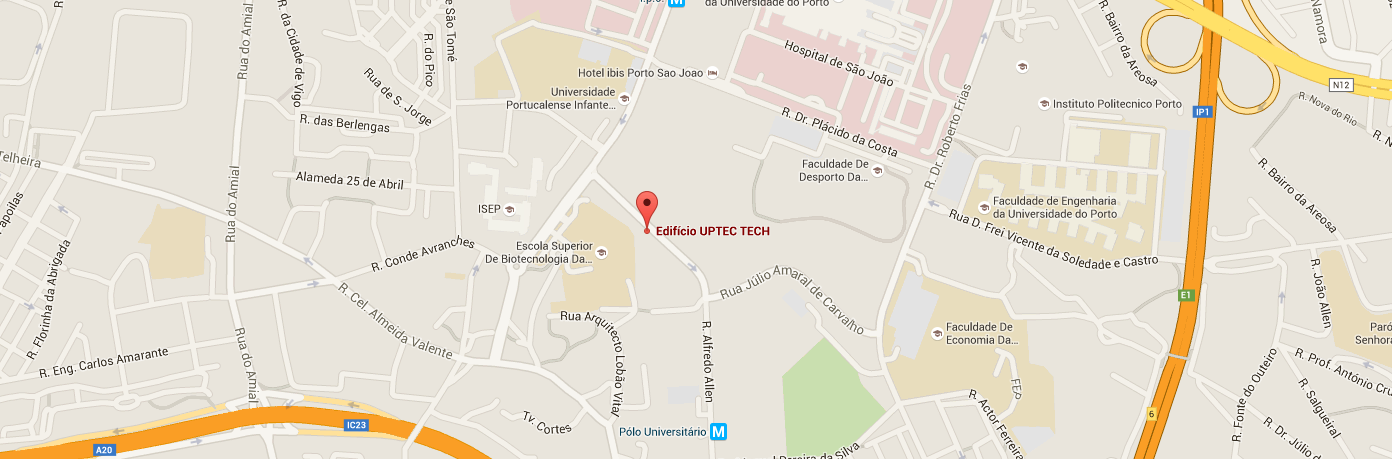
\includegraphics [scale=0.35]{location.png}

\newpage

\chapter{O Projeto}
\section{Descrição}
O projeto consiste na realização de um website para a U.Project. Este destina-se não só a publicitar a organização ao público, mas também a ajudar os integrantes desta a participarem nas suas atividades. Para isso, o site conta com uma área privada,onde os membros e associados da U.Project podem comunicar entre si,gerir os seus projetos e eventos ou tratar de outros assuntos relacionados com a mesma.

A direção possui também aqui uma ferramenta vital para facilitar o seu trabalho de gestão e controlo, desde os recursos humanos, até às notícias públicas e aos recursos financeiros da organização.

Espera-se que este projeto venha a contribuir para um aumento significativo da visibilidade da U.Project em Portugal e no mundo, permitindo assim alcançar os seus objetivos.
\section{Objetivos}
No Final do desenvolvimento do website,este tem que fazer o seguinte:
\begin{itemize}
\item Criar um website para a empresa U.Project;
\item Ser um website funcional;
\item O website tem que ser capaz de resgistar um visitante à base de dados;
\item O website tem que ter capacidade de fazer login a utilizadores;
\item O website tem que ser capaz de increver um utilizador nas atividades que irão decorrer;
\item Um utilizador com permissões suficientes tem que ser capaz de alterar as páginas a que tem acesso;
\item Um utilizador com permissões suficientes tem que ser capaz de alterar o sistema de pontos onde a partir disso os candidatos são classificados;
\item Um utilizador com permissões suficientes tem que ser capaz de alterar e adicionar projetos;
\item Um utilizador com permissões suficientes tem que ser capaz de alterar e adicionar departamentos;
\item Um utilizador com permissões suficientes tem que ser capaz de alterar e adicionar despesas;
\item Um utilizador tem que conseguir convidar amigos, de receber e enviar mensagens apartir de um chat localizado no website;
\item Um utilizador tem ser capaz de alterar as informações basicas sobre o mesmo;
\item Um utilizador tem que conseguir executar um pagamento de quotas e taxas;
\item O servidor tem que ser capaz de fornecer maneiras do utilizador recuperar a password esquecida;
\item Um utilizador tem que ser capaz de se inscrever para ser recrutado para trabalhar na empresa;
\item Um utilizador com permissões suficientes tem que ser capaz de aceitar ou recusar os utilizadores incritos;
\item Um utilizador tem que conseguir pesquisar sobre o que o mesmo queira saber;
\item O sistema tem estar sempre online nos dias da U.Project Acadamy para ter a certeza que os resultados são publicados;
\item O sistema tem ser capaz de continuar a funcionar quando ocorre um erro;
\item O sistema tem que ser capaz de fazer uma copia de segurança uma vez por dia;
\item O sistema tem que ser capaz de reniciar para evitar que o sistema sobrecarregue.
\item O website tem que ser um website dinamico e responsivo;
\item O webstite 
\end{itemize}
\section{Funcionalidades}
\begin{itemize}
\item Formulário de Contacto;
\item Newsletter;
\item Interação com redes sociais;
\item Acesso restrito ao login;
\item Parte administrativa com capacidade de alterar qualquer página que o utilizador tenha permissão;
\item Slideshow na página inicial;
\item Página de notícias;
\item Página de eventos a decorrer e eventos futuros;
\item Interação com o google maps;
\item Chat para comunicação entre amigos;
\item Interação com os departamentos e possibilidade de se inscrever.
\end{itemize}
\section{Ferramentas a utilizar}
\begin{itemize}
\item O Microsoft Word é uma ferramenta de processamento de texto,este programa permite criar documentos profissionais desde de currículos, folhas de rosto, a manuais. 
É uma ferramenta muito utilizada por escolas, universidades, empresas porque o word para além de uma ferramenta de processamento de texto pode alterar a formatação do texto, colocar o número de pagina, criar tabelas.
\begin{figure}
\centering

\includegraphics[width=0.1\textwidth]{word_logo.png}
\caption{Logotipo do Microsoft Word}
\end{figure}

\item O Enterprise Architect é programa de manuseamento de informação e invovar no mundo complexo e exigente de hoje, este programa serve para criar por exemplo: um modelo da base de dados a ser construida, criar um mapa de um website.
\begin{figure}
\centering

\includegraphics[width=0.5\textwidth]{Enterprise_Architect.png}
\caption{Logotipo do Enterprise Architect}
\end{figure}

\item Adobe PhotoShop é um programa criado e desenvolvido por Thomas Knoll.
É um dos melhores programas que existe para alterar imagens, no entanto, também está cada vez mais a ser utilizado para produzir imagens na Internet. A versão mais atual é a "Photoshop CS3", esta versão é utilizada principalmente por profissionais.
\begin{figure}
\centering

\includegraphics{Photoshop.jpg}
\caption{Logotipo do photoshop}
\end{figure}

\item O Notepad++ é o editor de texto muito completo e avançado, que pode fácilmente ser usado como um bloco de notas.
A diferença entre o Notepad do windows e o notepad++ é que este ultimo pode ser utilizado em programação, uma vez que permite várias linguagens de programação.
\begin{figure}
\centering

\includegraphics{note.jpg}
\caption{Logotipo do Notepad++}
\end{figure}

\item LaTeX é um programa utilizado mais para documentos mais proficionais, é mais utilizado em empresas e univerisidades, este programa é um conjunto de macros e marcações, o LaTeX é um programa muito diferente do word pois este é mais detalhado.
\begin{figure}
\centering

\includegraphics{LaTeX.png}
\caption{Logotipo do LaTeX}
\end{figure}

\item O GitHub é um repositorio onde podemos hospedar os nossos projetos, este programa é muito util quando é um projeto realizado em equipa, pois este programa mantem todos os ficheiro sempre atualizados. 
\begin{figure}
\centering

\includegraphics{Git.png}
\caption{Logotipo do GitHub}
\end{figure}
\end{itemize}

\linebreak
\newpage
\section{Atividades a desenvolver}
\addcontentsline{toc}{chapter}{Atividades a desenvolver}
Actors é um diagrama em que cada pessoa pode representar a sua própria pessoa, organização ou sistema externo que pode interagir com o sistema definindo assim as suas permissões.

User stories é uma definição de alto nível de exigência, contendo todas as informações para tornar possível uma estimativa do esforço necessário para poder implementar uma função. Normalmente uma User Story é descrita pelo seguinte modelo: 
Com um (papel) eu pretendo (algo) para que eu (beneficio).

Interface do website pretende dar uma perspetiva de um protótipo de como o produto final deverá ficar, que servirá como base para o design.

Sitemap é uma lista com todas as páginas (URLs) do site, funciona como uma espécie de mapa que irá ajudar e guiar motores de busca ou utilizadores a navegar e encontrar páginas do site.

As interações fundamentais, também é um bem  no planeamento que o sistema deverá obedecer para ilustrar a sequência de etapas associadas a cada um dos cenários.
Estes diagramas não podem conter todos os detalhes de interação, mas eles devem fornecer uma experiência completa de como será os passos para chegar ao objetivo final.


Requisitos do sistema nesta etapa prever-se todos os requisitos obrigatórios para que a empresa e o seu website funcionem sem qualquer problemas no futuro.

Modelo conceptual UML tem como função ajudar a planear a base de dados, contendo benefícios como poder representar notas e restrições adicionais no diagrama.

\section{Calendarização do Projeto}

\section{Fases de Implementação}
\addcontentsline{toc}{chapter}{Fases de Implementação}

\subsection{A2a - Actors}
	Actors, que é um diagrama em que cada pessoa representa uma pessoa, organização ou sistema externo que pode interagir com o sistema definindo assim as suas permissões, como ilustrado no anexo 1.
\subsection{A2b - User Stories}
	User Stories, que é uma definição de alto nível de exigência, contendo todas as informações para tornar possível uma estimativa do esforço necessário para poder implementar uma função. 
	
	Normalmente uma User Story é descrita pelo seguinte modelo: 
	
Com um (papel) eu pretendo (algo) para que eu (beneficio).

Ex: Como Utilizador quero pesquisar toda a informação pública, para poder estar facilmente a par das notícias e eventos da organização que me interessam.

Ex nº2 :Como Utilizador pretendo saber quais são os projetos nos quais a U.Project esteve envolvida ou está a planear para poder avaliar se vale a pena ser um associado.

Ex nº3: Visitante pretendo efetuar login para poder aceder à área reservada do website.

\subsection{A3a - Interface do Website}
Esta parte do nosso planeamento, pretende dar uma perspetiva de um protótipo de como o produto final deverá ficar, como ilustrado nas figuras dos anexos 2 até 5.

\subsection{A3b - Sitemap}
	
Utilizando o programa Architect Enterprise criamos um modelo sitemap do website, ou seja, cada Caixa significa uma página no website, como ilustrado no anexo 6

\subsection{A3c - Interações}
	
Nesta secção é descrito as interações fundamentais que o sistema deverá obedecer para ilustrar a sequência de etapas associadas a cada um dos cenários.

Estes diagramas não podem conter todos os detalhes de interação, mas eles devem fornecer uma experiência completa de como será os passos para chegar ao objetivo final.


\begin{itemize}
		\item Cenario 1: Página de atividades - Anexo: 7
		\item Cenario 2: Página de adicionar/editar utilizadores - Anexo: 8
		\item Cenario 3: Página de adicionar/editar parceiros - Anexo: 9
		\item Cenario 4: Página de adicionar/editar sistema de pontos - Anexo: 10
		\item Cenario 5: Página de adicionar/editar projetos - Anexo: 11
		\item Cenario 6: Página de adicionar/editar departamentos - Anexo: 12
		\item Cenario 7: Página das despesas - Anexo: 13
		\item Cenario 8: Página de Amigos - Anexo: 14
		\item Cenario 9: Todas as interações possíveis da parte da administração - Anexo: 15
		\item Cenario 10: Login - Anexo: 16	
		\item Cenario 11: Página de gerir páginas - Anexo: 17	
		\item Cenario 12: Página de gestão de compras - Anexo: 18
		\item Cenario 13: Página de recuperar Password - Anexo: 19	
		\item Cenario 14: Página do formulário de  Recrutamento - Anexo: 20	
		\item Cenario 15: Registo - Anexo: 21	
		\item Cenario 16: Procura - Anexo: 22	
		\item Cenario 17: Seleção de candidatos - Anexo: 23
		\item Cenario 18: Página Perfil de Utilizador - Anexo: 25
		\item Cenario 19: Quotas - Anexo: 24
\end{itemize}		
\subsection{A4 - Requisitos do sistema}
	
	
	Nesta etapa tivemos que em todos os requisitos obrigatórios para que a empresa e o seu website funcionassem sem qualquer problemas no futuro, como ilustrado no anexo 26, 27, 28.

\subsection{A5 - Modelo UML}
	
	Um dos passos mais importantes a planear é o modelo da base de dados, para isso utilizasse o Modelo conceptual UML que tem como benefícios poder representar notas e restrições adicionais no diagrama, como ilustrado no anexo 29.

\subsection{Especificação de Requisitos}

Os requisitos especificados eram basicamente que qualquer vistante do website da U.Project tivesse imediatamente á sua disposição as noticias base da empresa e a sua descrição, tal como os contactos dos responsáveis e localização da sede da empresa.

Permitir que um utilizador se registe para possuir um perfil editável e poder aceder a outras informações.

Só um utilizador registado tem acesso ás informações restritas.

Um grupo de administradores e head-admins para gerir o website e membros.

Permitir o gerenciamento do website apartir do Gestor PhP My Admin com linguagem SQL.

\chapter{Considerações Finais}

\section{Dificuldades}
Durante a elaboração deste projeto houveram várias dificuldades que atrasaram de certa forma o trabalho da equipa.
Um dos principais problemas ocorridos foi, sem dúvida, a coordenação e cooperação entre os grupos. Reunimos várias vezes o grupo com o objetivo de melhorar nestes aspectos e aumentar a velocidade de trabalho.
Um outro ponto negativo foi a dificuldade na escolha de um layout para o website que foi, de certa forma, resolvido com a evolução da cooperação entre os grupos.
Por fim, a interpretação do código e o uso de ferramentas que antes não conhecíamos foi um outo grande problema, onde tentamos aprender e melhorar apartir de tutoriais disponibilizados na internet. Quando esses tutoriais não satisfaziam as necessidades do grupo procuramos ajuda junto do Márcio Fontes.
\newpage

\chapter*{Bibliografia}



\chapter*{Anexos}
\subsection{A2}
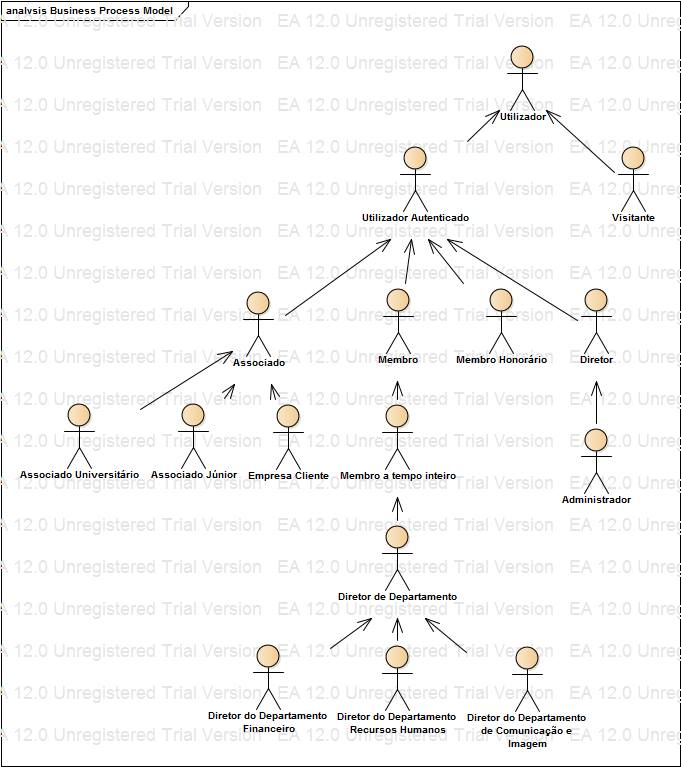
\includegraphics[\linewidth, height=5cm]{atores.png} 

\caption{Figura 1: Atores}

\subsection{A3A}


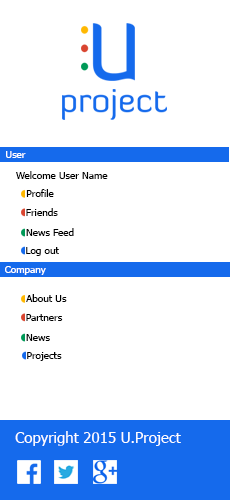
\includegraphics[\linewidth, height=5cm]{Mobile.png} 

\caption{Figura 2: Layout do Menu Mobile}



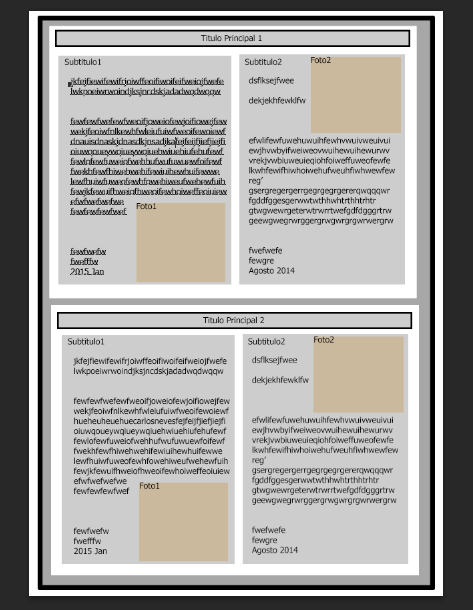
\includegraphics[\linewidth, height=5cm]{Noticias.PNG} 

\caption{Figura 3: Layout das noticias}



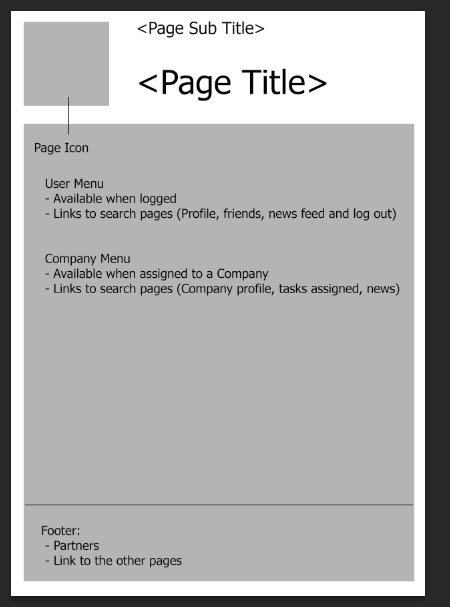
\includegraphics[\linewidth, height=5cm]{Pagina.PNG} 

\caption{Figura 4: Layout do utilizador}



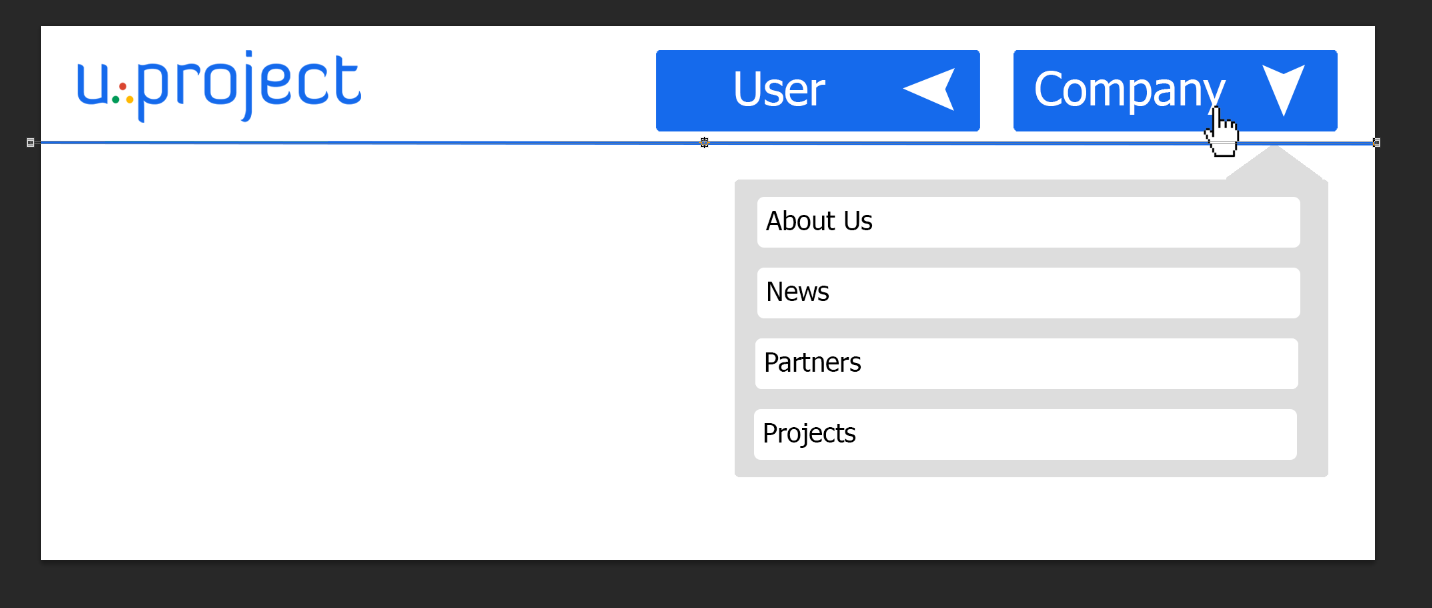
\includegraphics[\linewidth, height=5cm]{Pc.PNG} 

\caption{Figura 5: Layout do header}


Nas imagens acima estão presentes os diferentes protótipos para os layouts deste {\it website}.

Na primeira imagem, encontra-se o protótipo do menu lateral da versão {\it mobile} do site, a segunda e terceira, os protótipos das páginas de notícias e de utilizador e a quarta imagem o protótipo do {\it header} do site no computador.

\subsection{A3B}


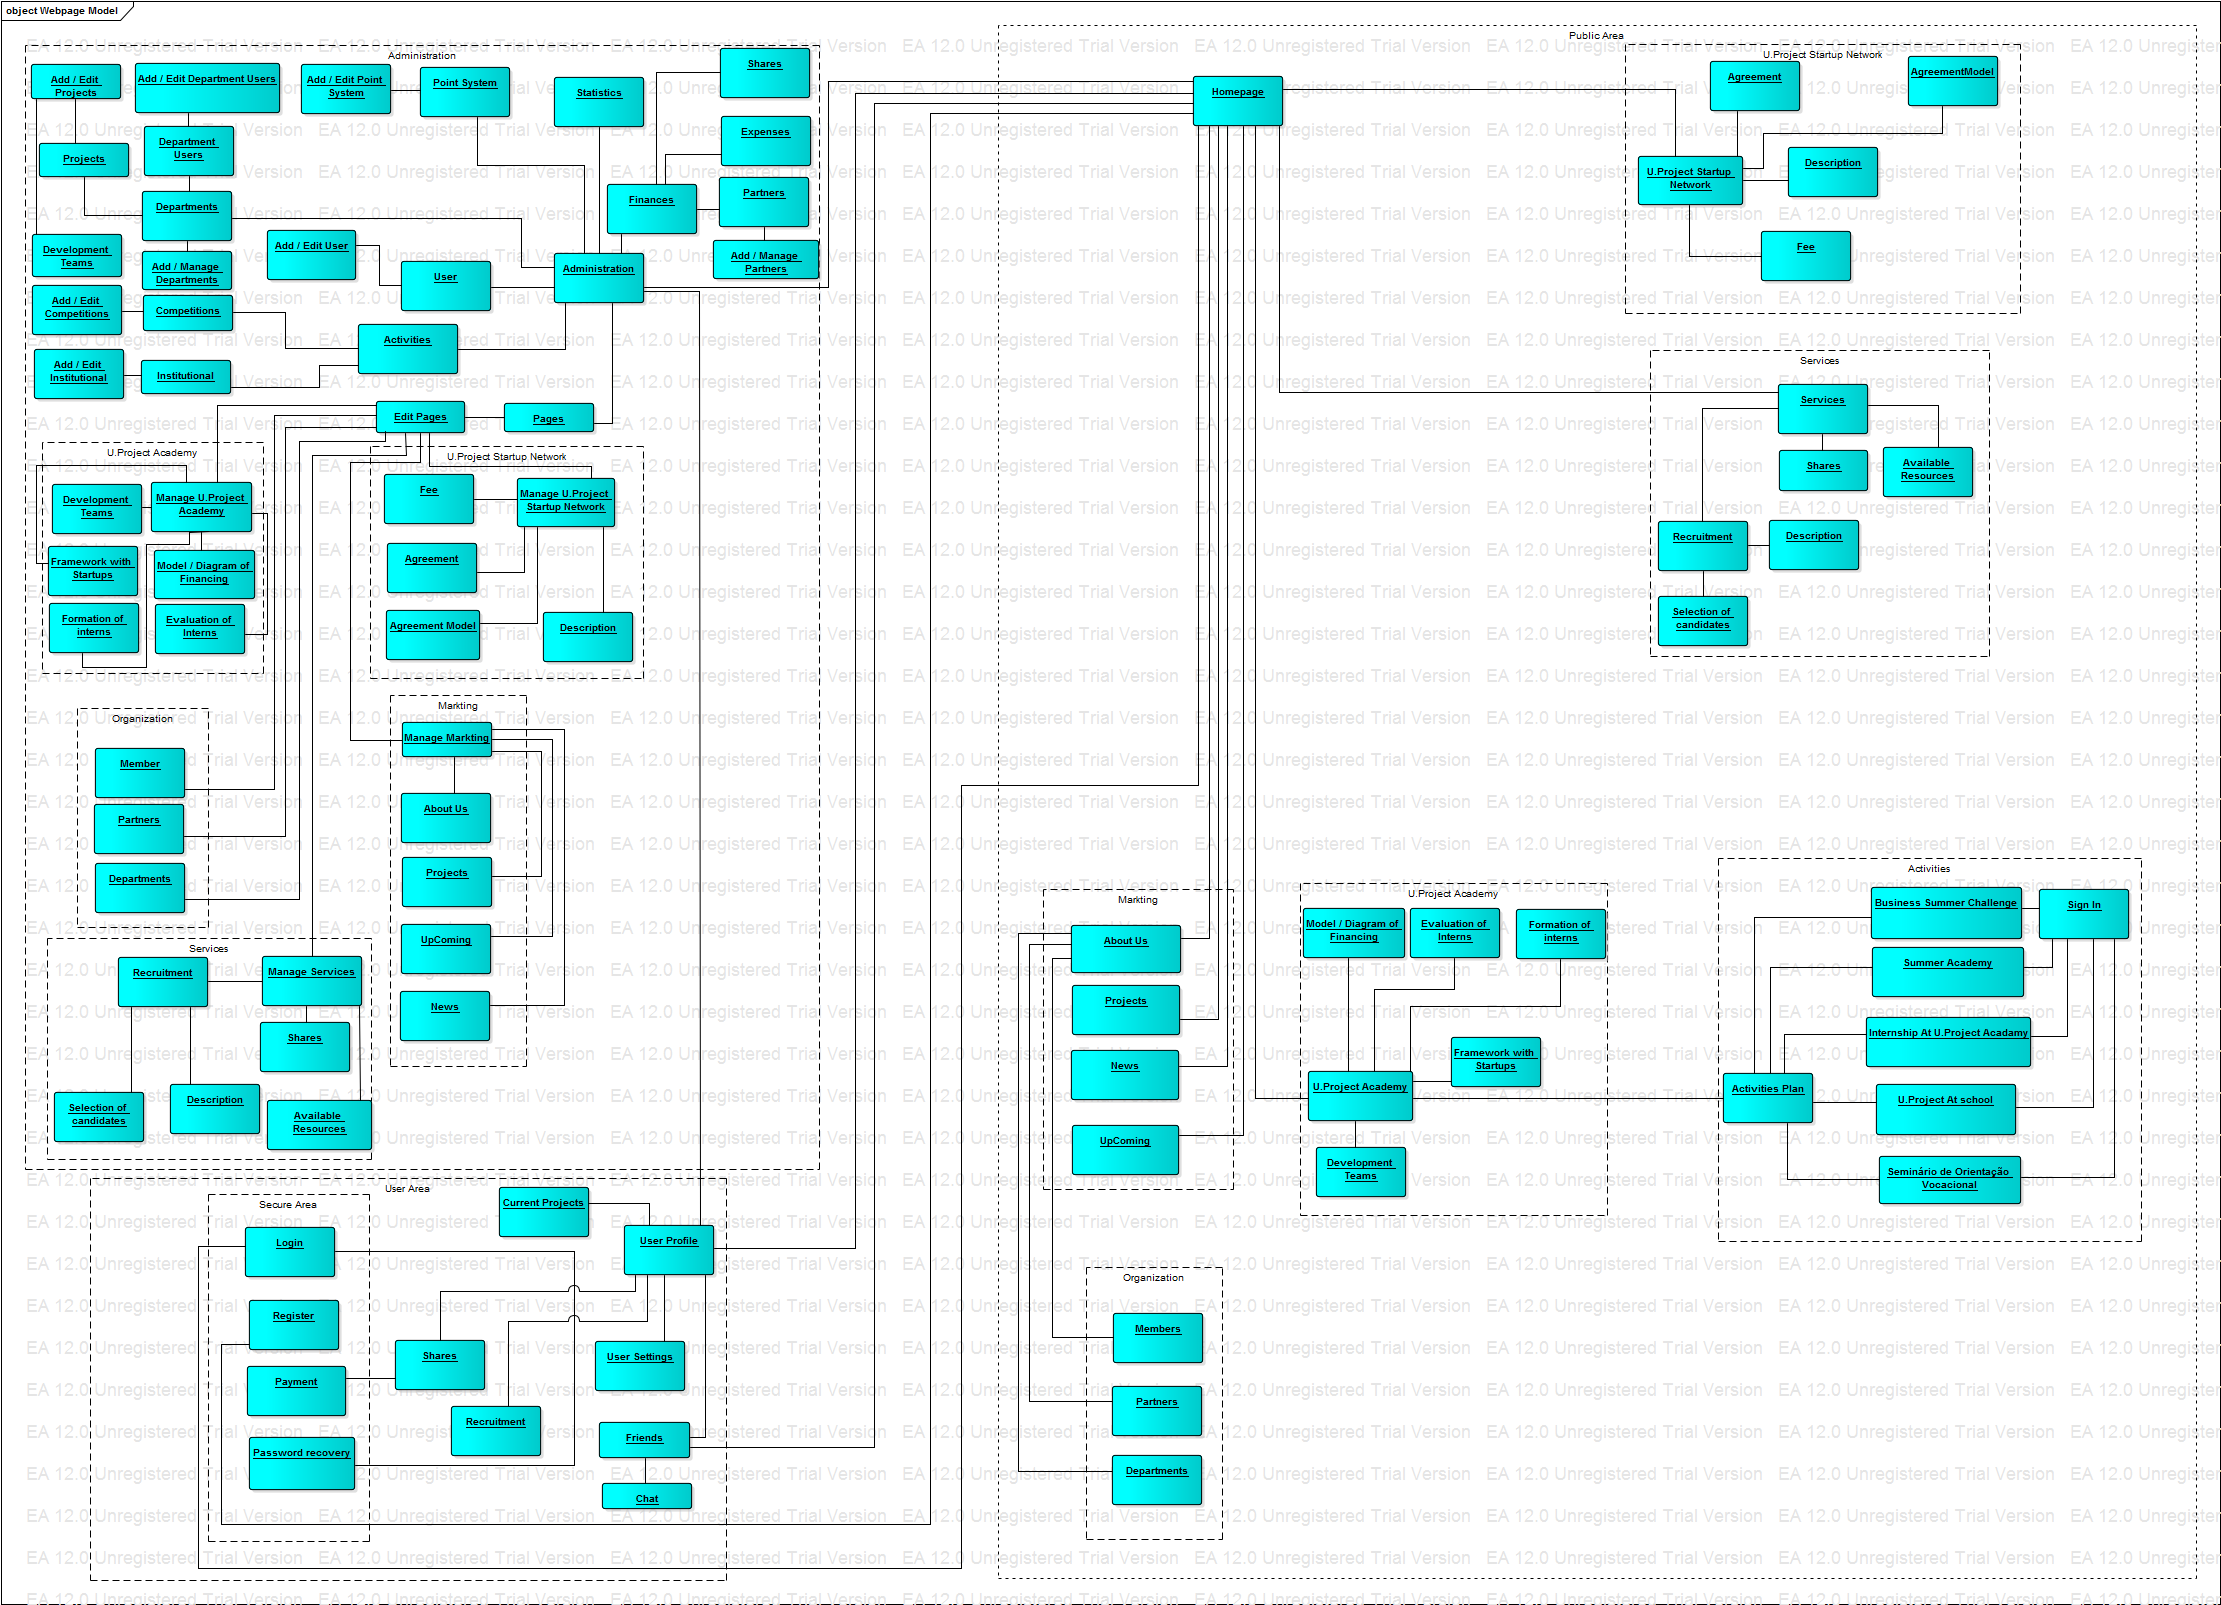
\includegraphics[width=1\linewidth, height=10cm]{Webpage_Model.png} 

\caption{Figura 6: Website Webpage Model}

Nesta imagem está presente o modelo que o {\it website} irá seguir.

\subsection{A3C}


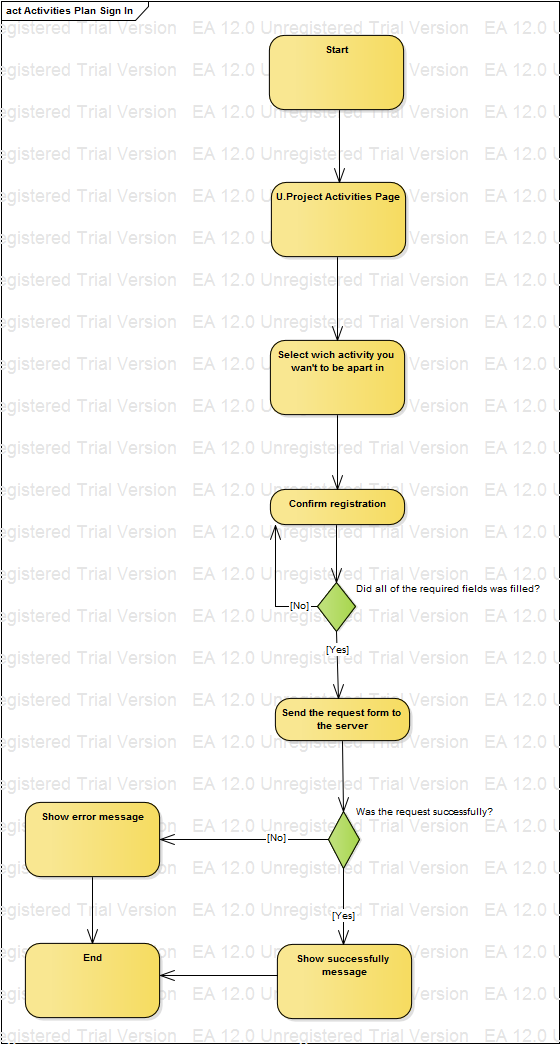
\includegraphics[\linewidth, height=10cm]{Activities_Plan_Sign_In.png} 

\caption{Figura 7: Inscrever-se nas atividades}



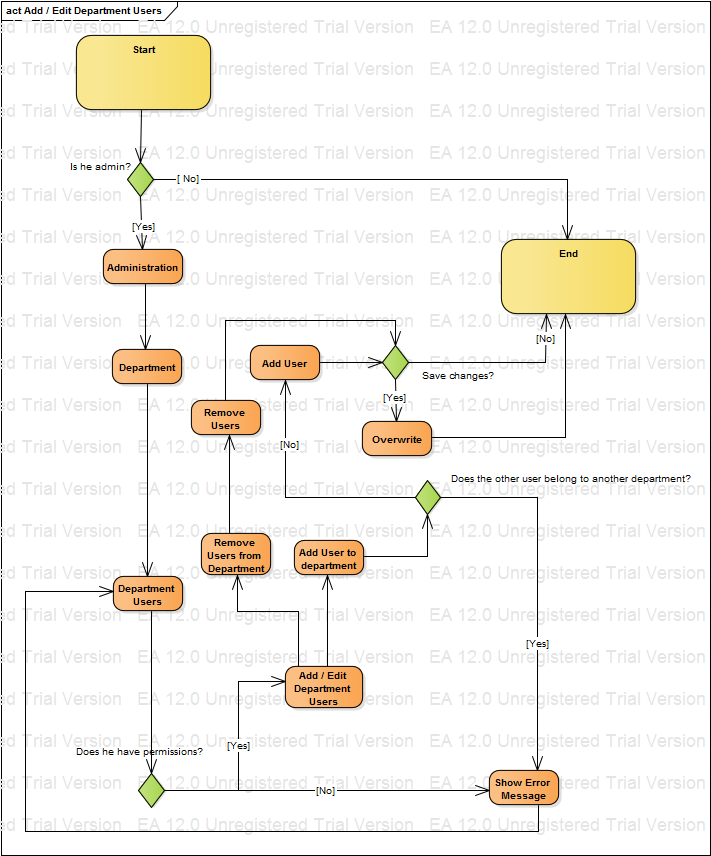
\includegraphics[\linewidth, height=5cm]{Add_Edit_Department_Users.png} 

\caption{Figura 8: Departamento dos Utilizadores}



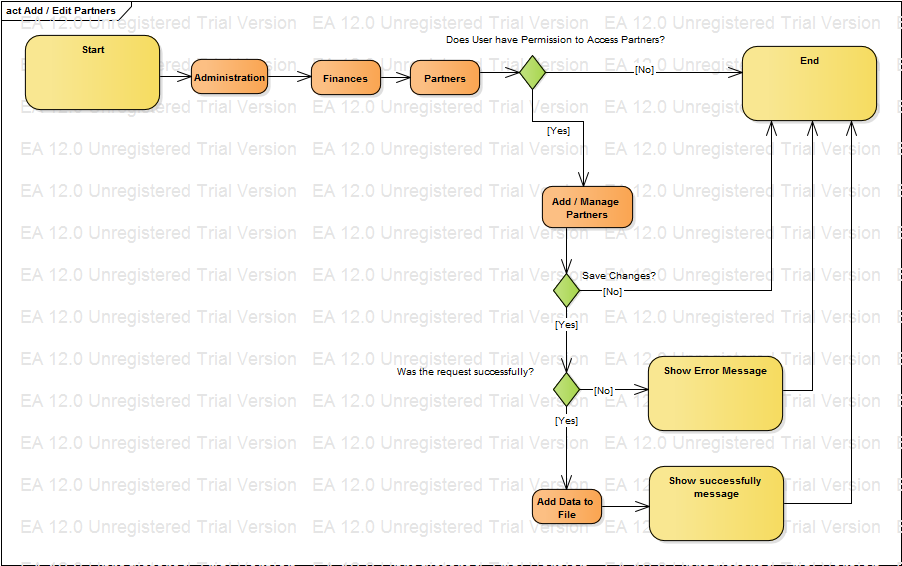
\includegraphics[\linewidth, height=5cm]{Add_Edit_Partners.png} 

\caption{Figura 9: Parceiros}



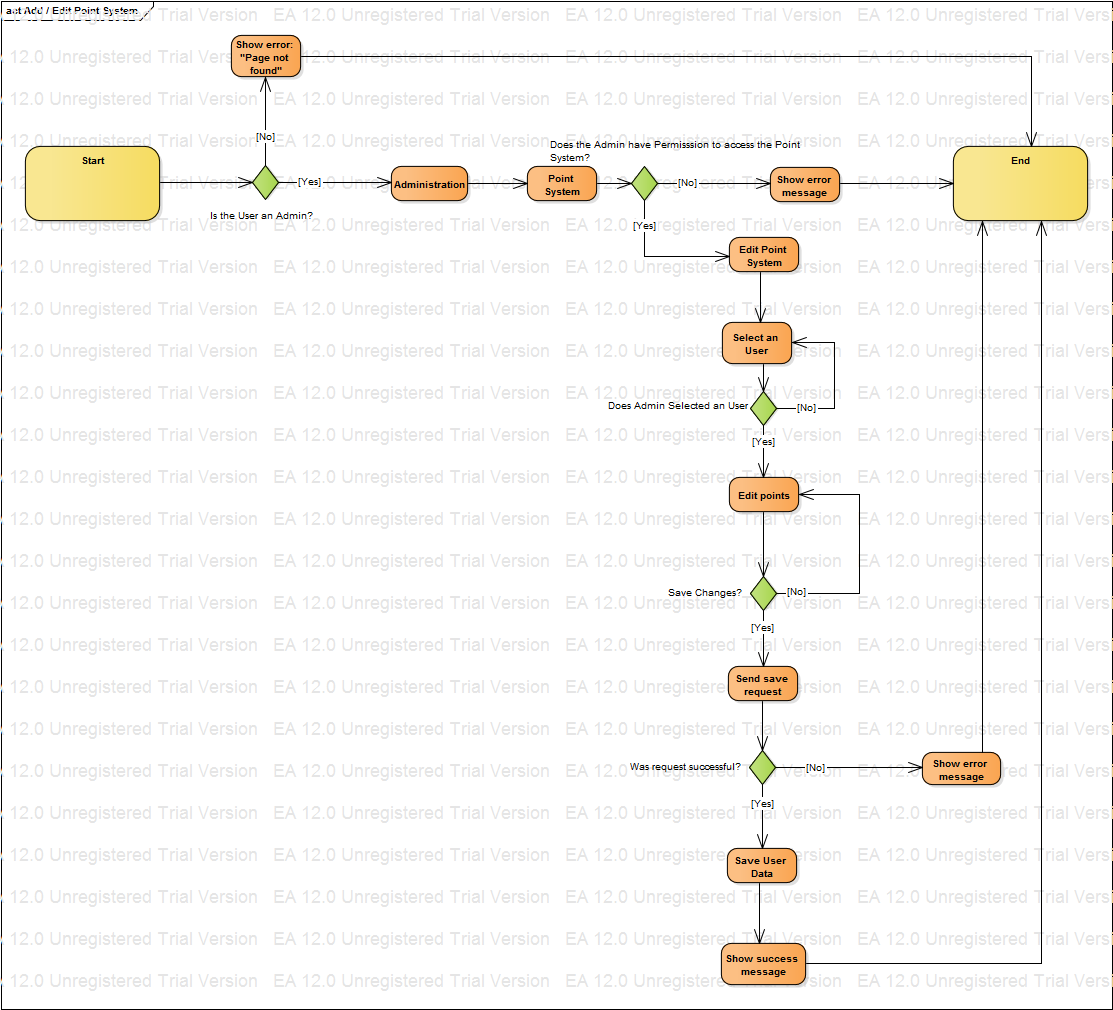
\includegraphics[\linewidth, height=5cm]{Add_Edit_Point_System.png} 

\caption{Figura 10: Sistema de pontos}



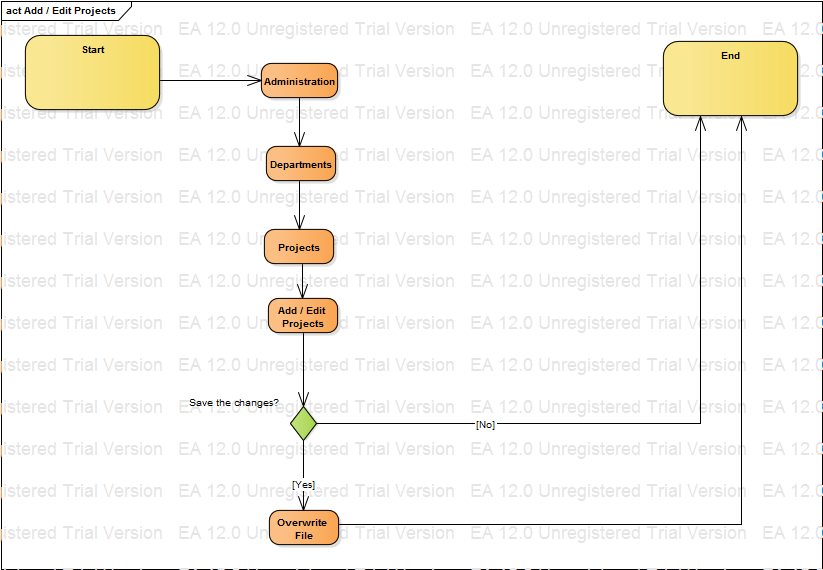
\includegraphics[\linewidth, height=5cm]{Add_Edit_Projects.png} 

\caption{Figura 11: Projetos}



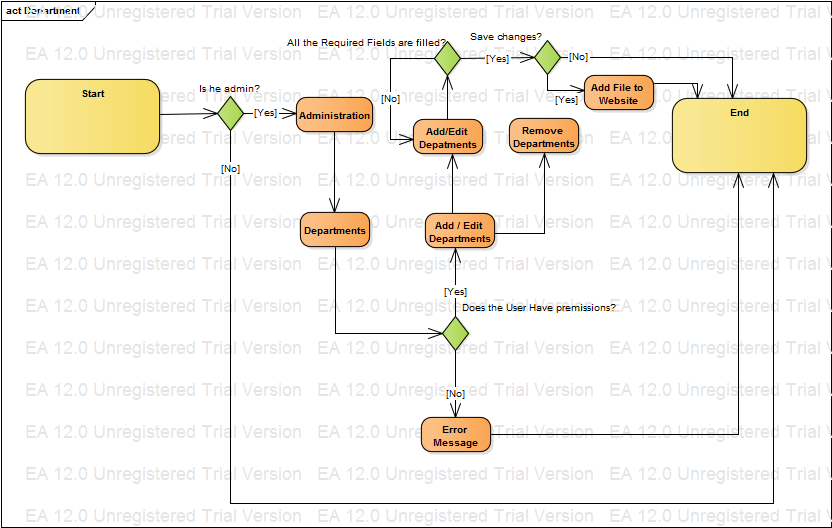
\includegraphics[\linewidth, height=5cm]{Department.png} 

\caption{Figura 12: Departamentos}



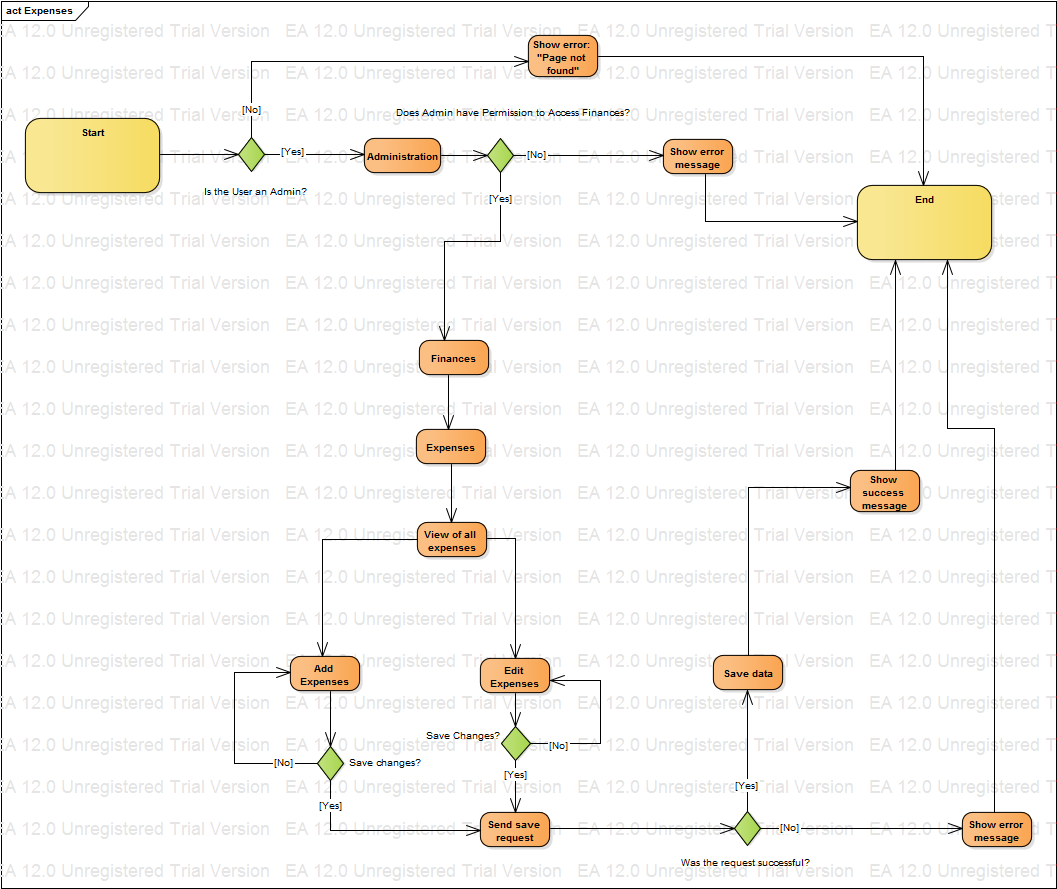
\includegraphics[\linewidth, height=5cm]{Expenses.png} 

\caption{Figura 13: Despesas}



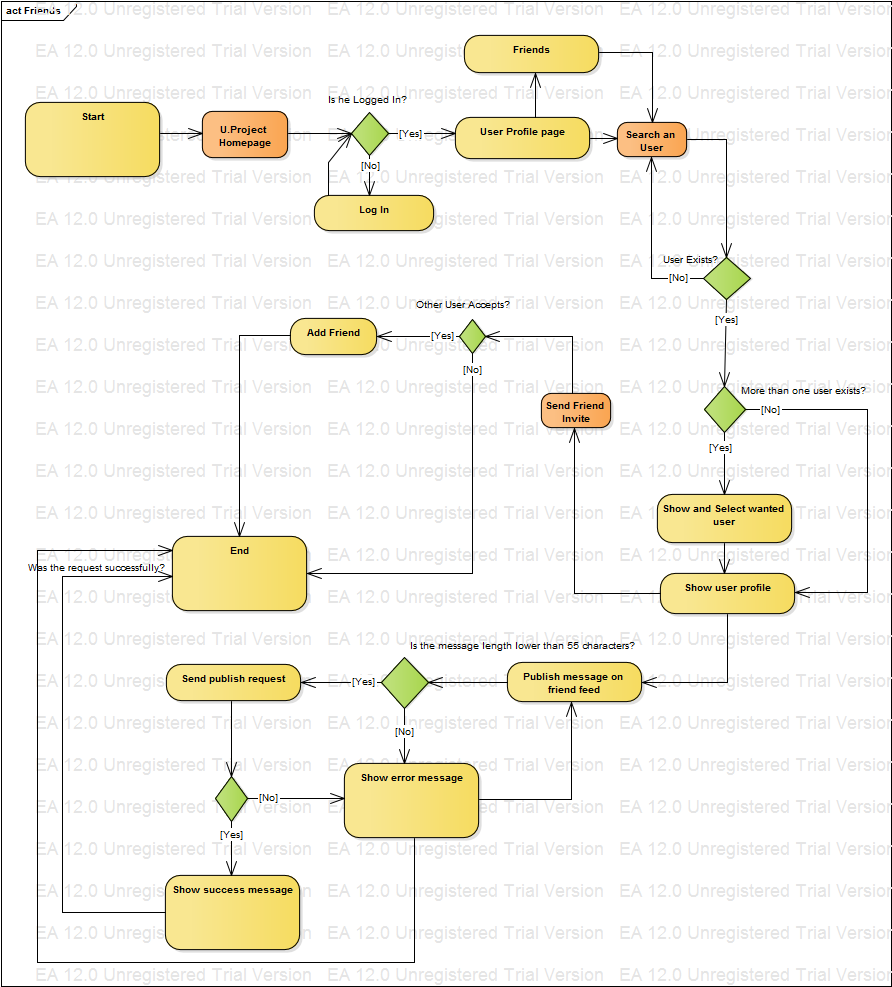
\includegraphics[\linewidth, height=5cm]{Friends.png} 

\caption{Figura 14: Amigos}


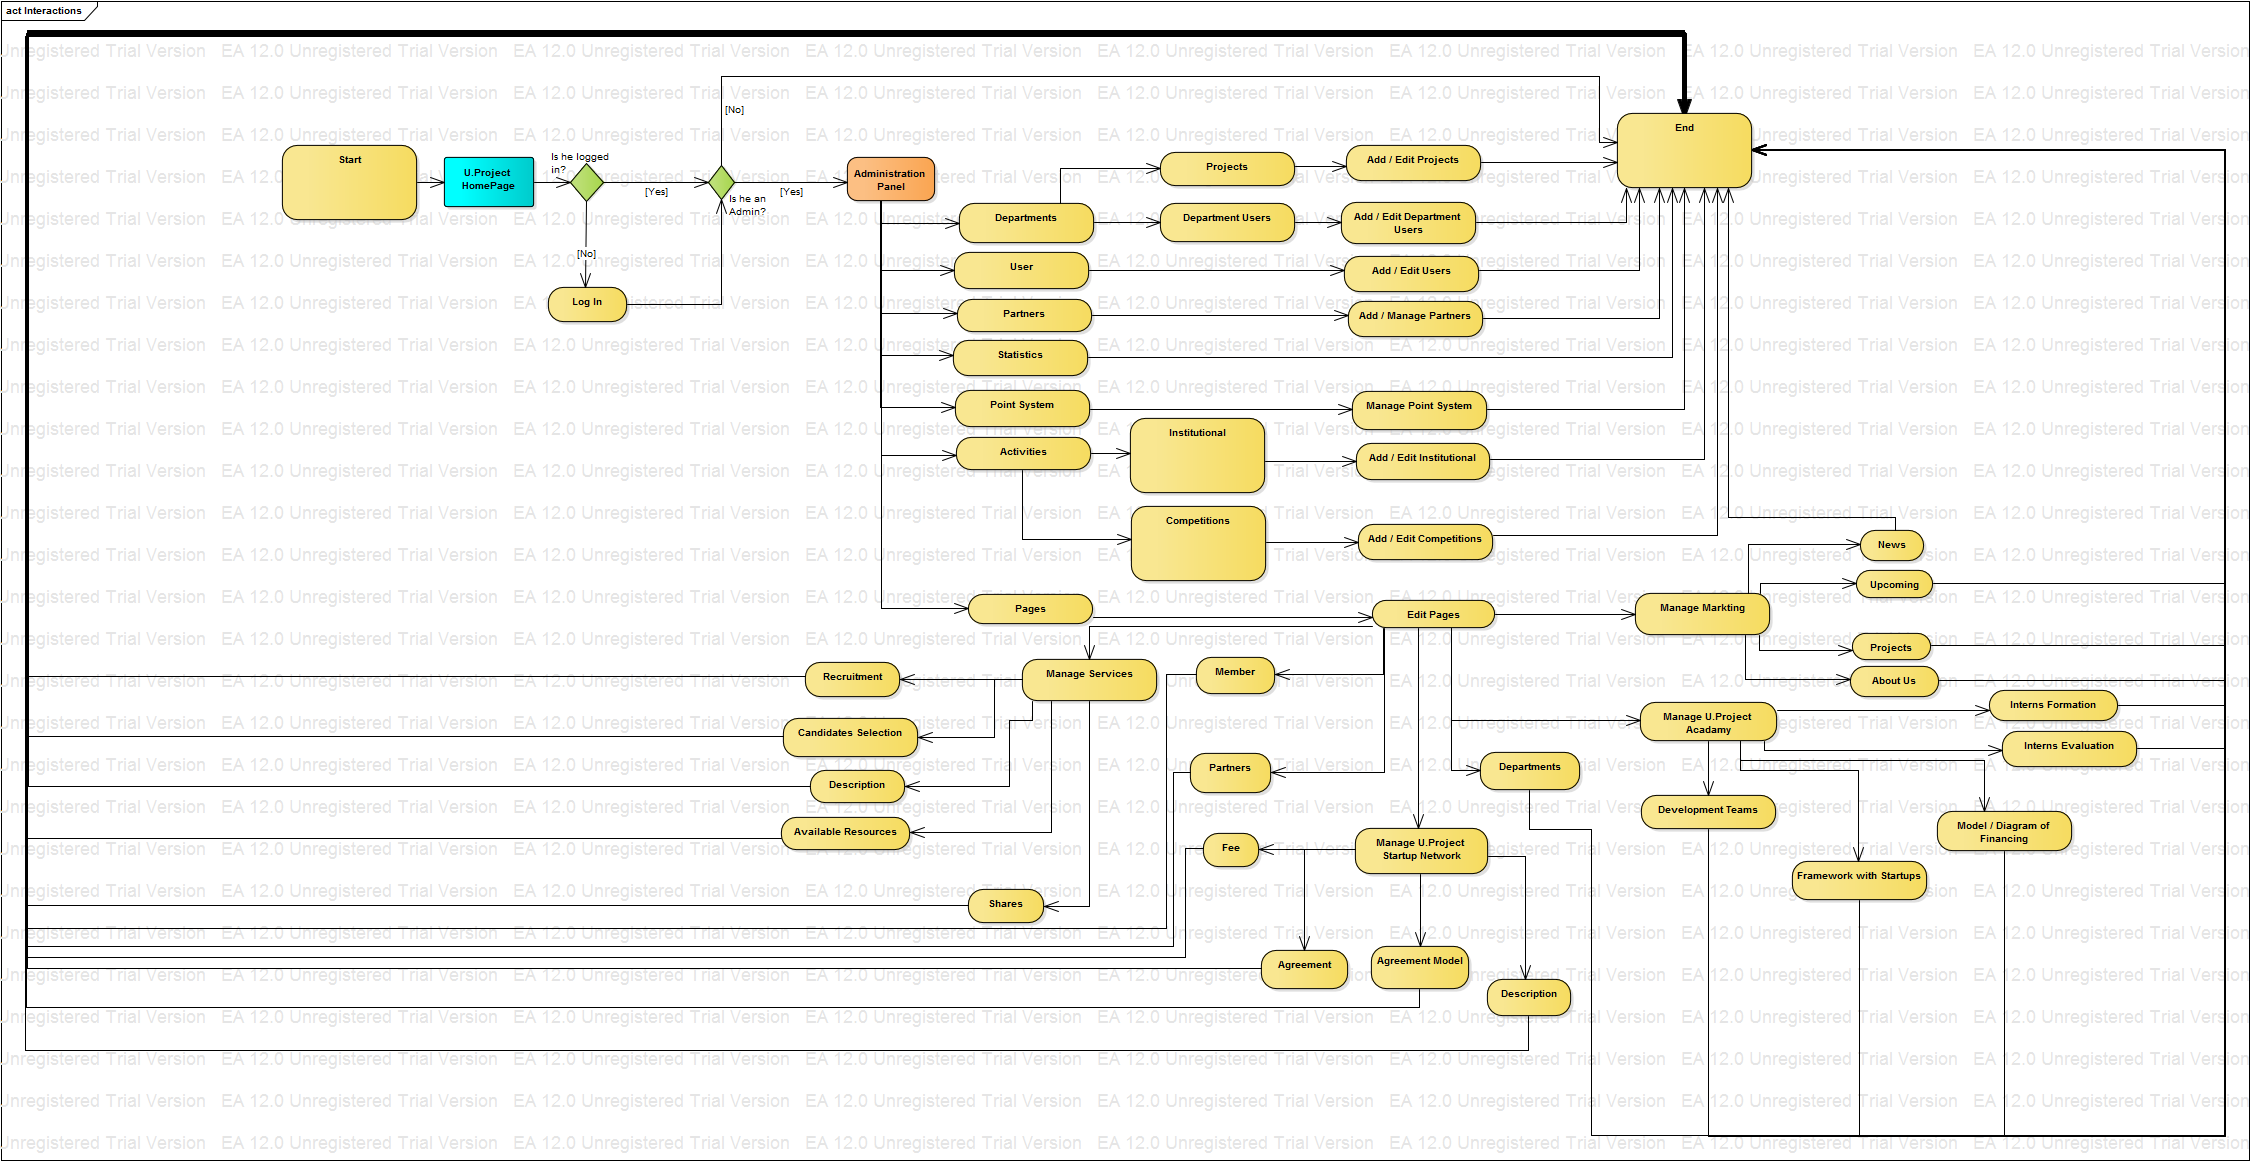
\includegraphics[\linewidth, height=5cm]{Interactions.png} 

\caption{Figura 15: Administração}



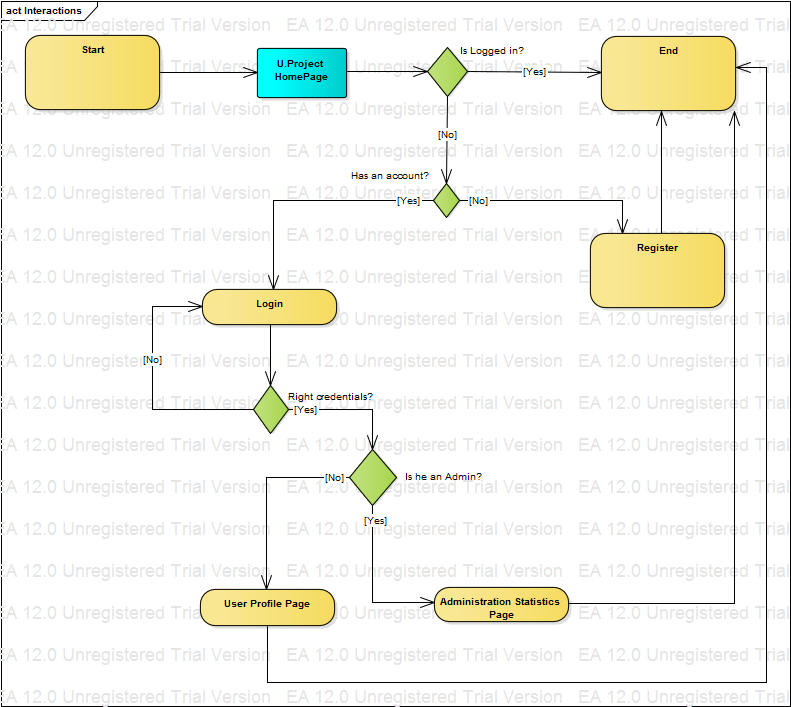
\includegraphics[\linewidth, height=5cm]{Login.png} 

\caption{Figura 16: Iniciar sessão}



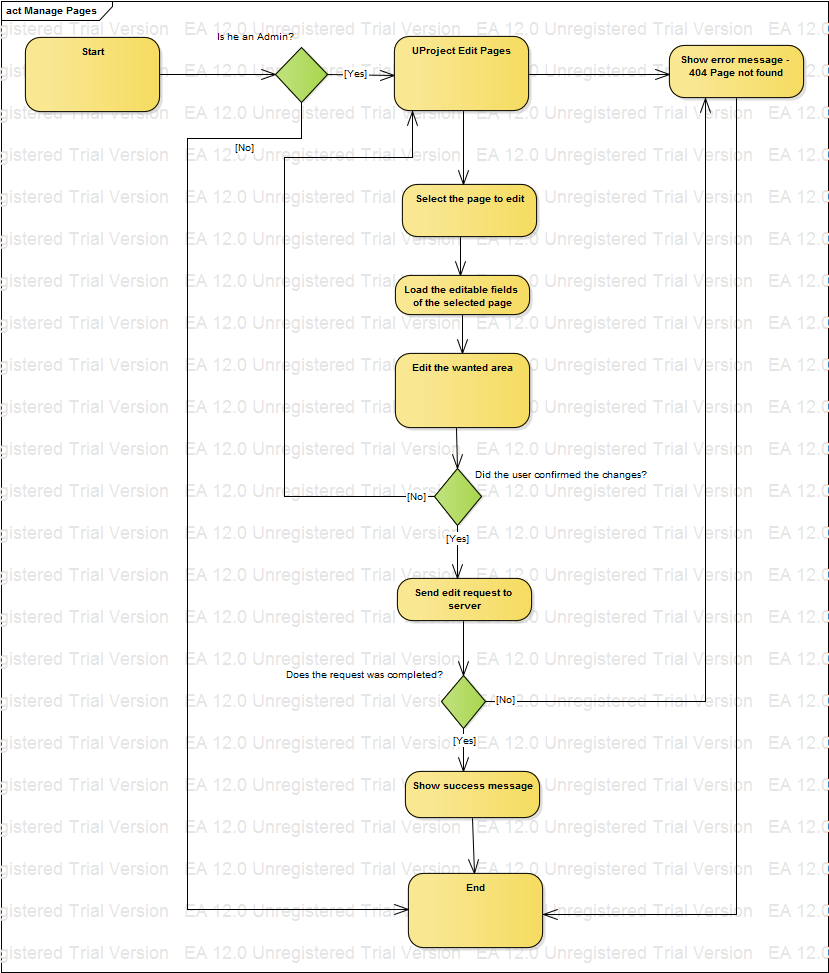
\includegraphics[\linewidth, height=5cm]{Manage_Pages.png} 

\caption{Figura 17: Gestão das paginas}



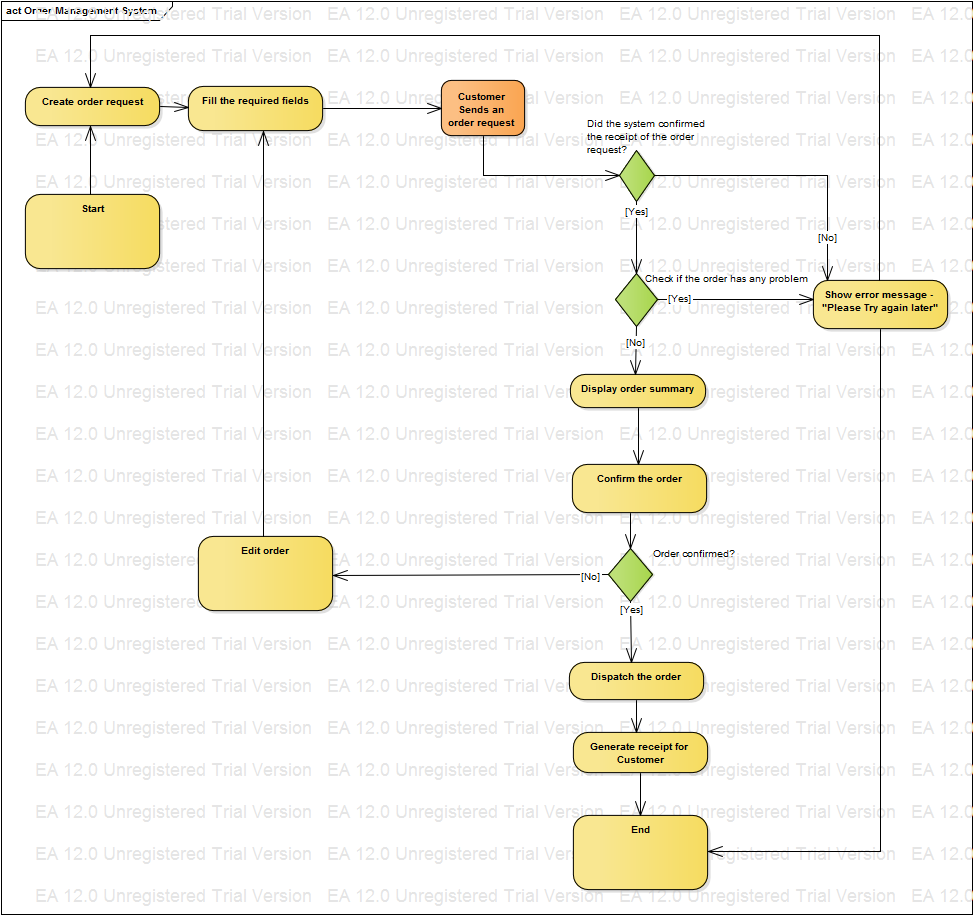
\includegraphics[\linewidth, height=5cm]{Order_Management_System.png} 

\caption{Figura 18: Sistema de gestão}



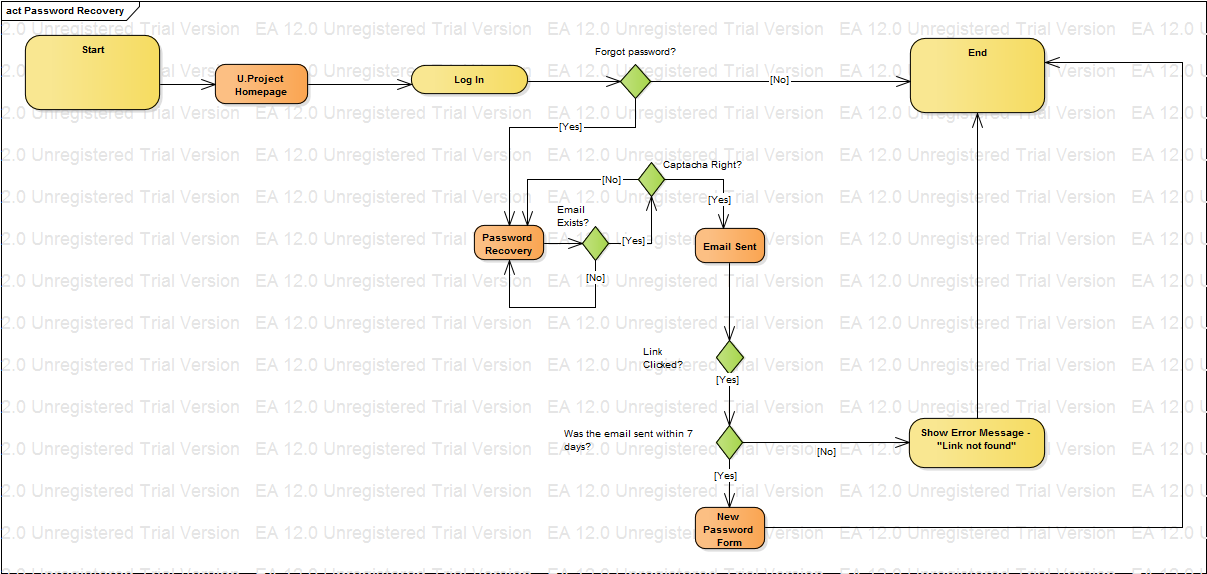
\includegraphics[\linewidth, height=5cm]{Password_Recovery.png} 

\caption{Figura 19: Recuperação da password}



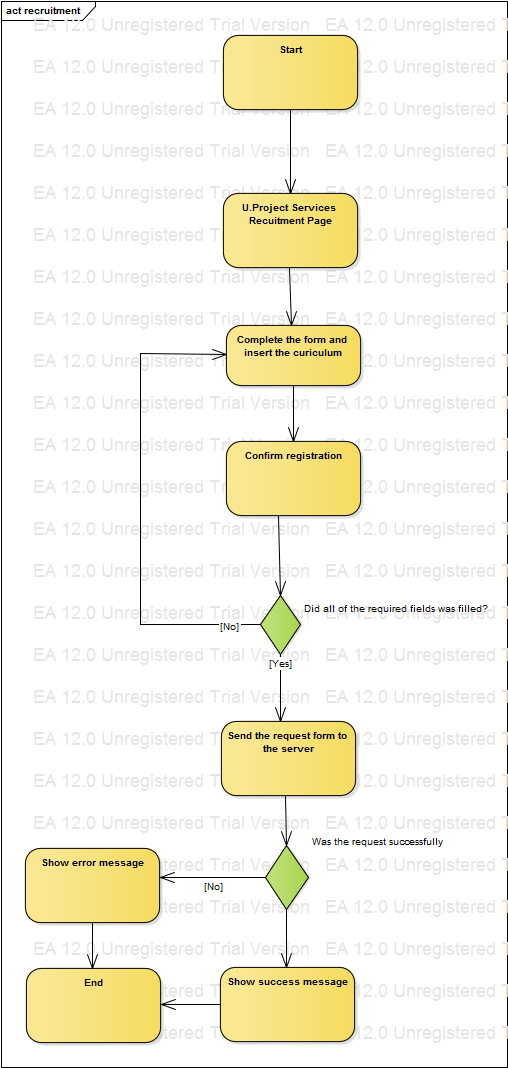
\includegraphics[\linewidth, height=5cm]{recruitment.png} 

\caption{Figura 20: Recrutamento}



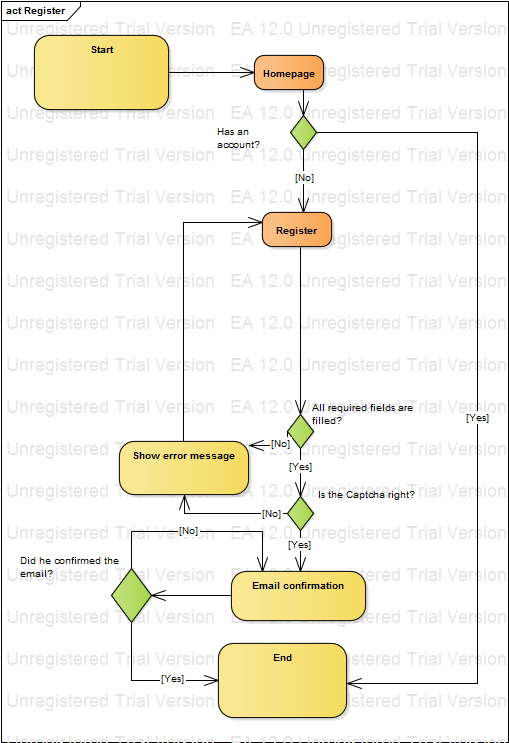
\includegraphics[\linewidth, height=5cm]{Register.png} 

\caption{Figura 21: Registar}



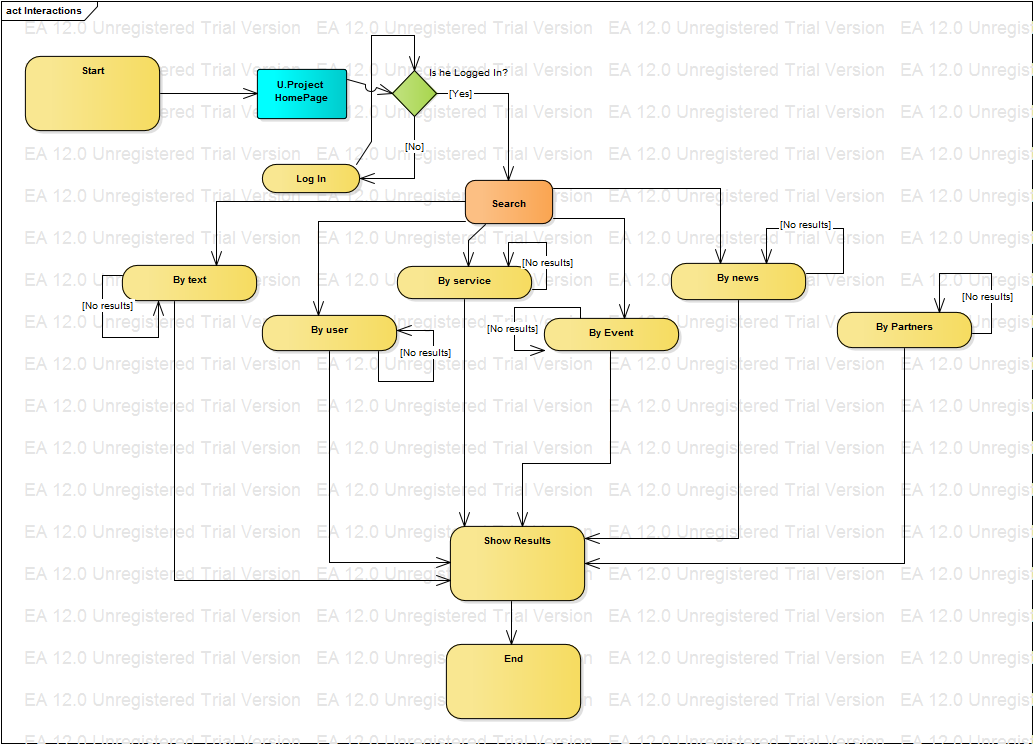
\includegraphics[\linewidth, height=5cm]{Search.png} 

\caption{Figura 22: Pesquisa}



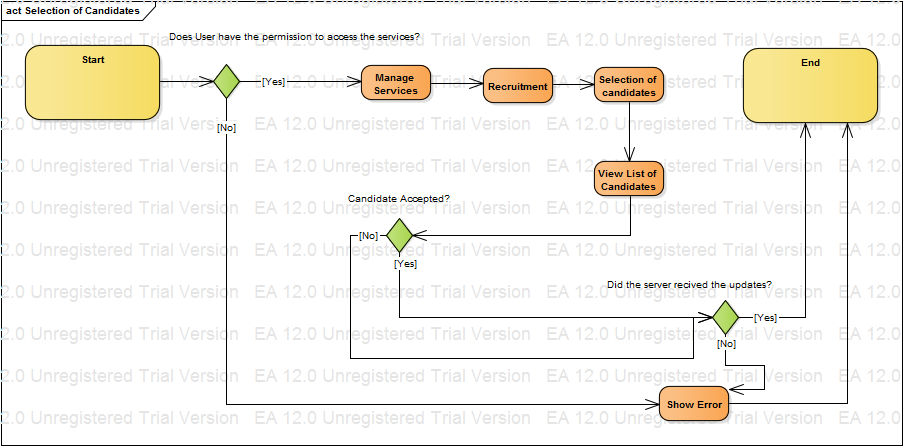
\includegraphics[\linewidth, height=5cm]{Selection_of_Candidates.png} 

\caption{Figura 23: Seleção dos canidatos}



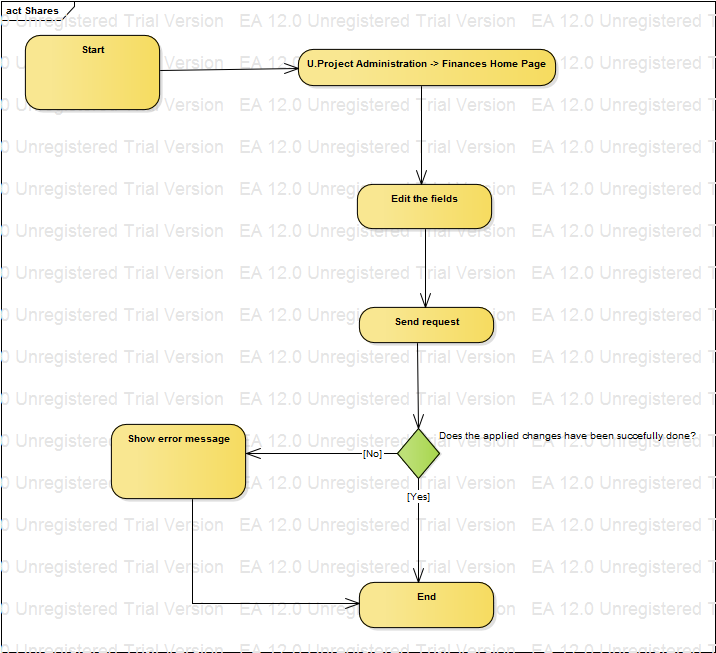
\includegraphics[\linewidth, height=5cm]{Shares.png} 

\caption{Figura 24: Quotas}



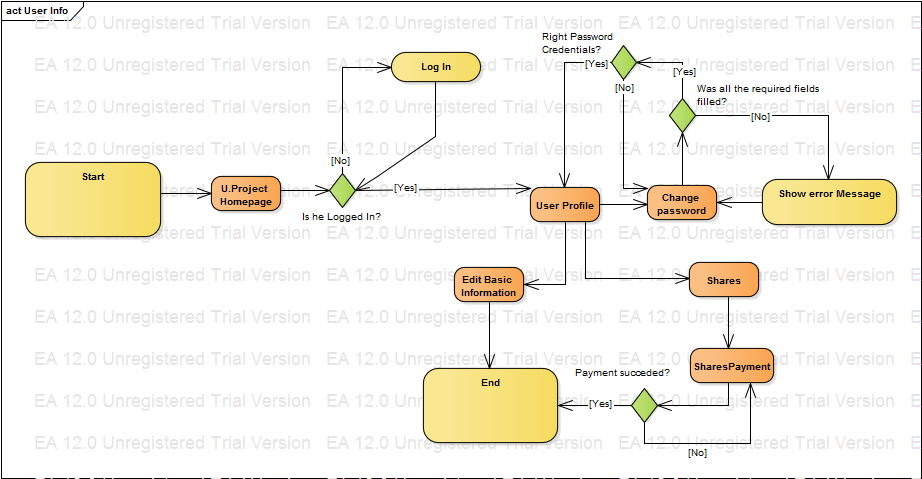
\includegraphics[\linewidth, height=5cm]{User_Info.png} 

\caption{Figura 25: Info do utilizador}

Nas imagens acima estão representadas as ações do {\it website} como, por exemplo, o {\it login}, o registo e a recuperação de palavras-passe.

Cada imagem dá uma explicação detalhada acerca do que acontece dentro do código do {\it website} quando é executada alguma das ações acima referidas.

\subsection{A4}


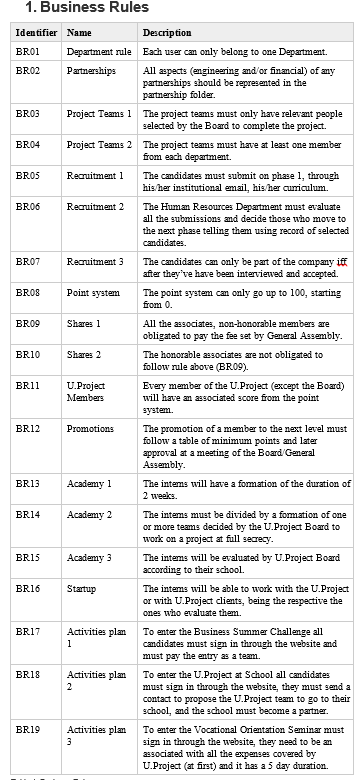
\includegraphics[\linewidth, height=5cm]{Business_rules.PNG} 

\caption{Figura 26: Regras de negócio}



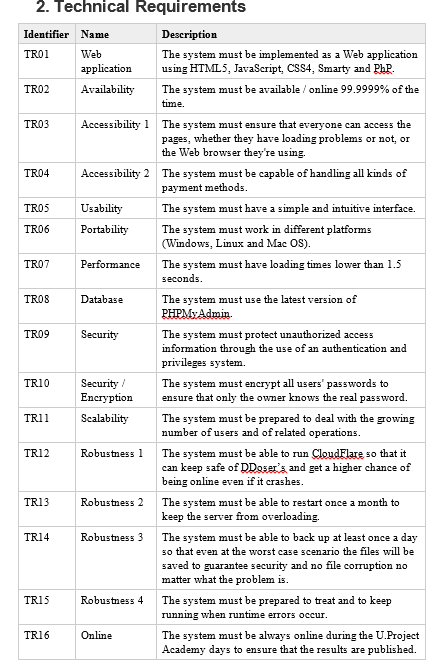
\includegraphics[height=5cm]{Technical_req.PNG} 

\caption{Figura 27: Requerimentos técnicos}



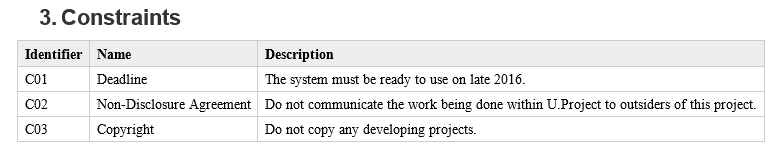
\includegraphics[width=1\linewidth]{Constraints.PNG} 

\caption{Figura 28: Restrições}

Nas imagens acima estão representadas as regras de negócio, requerimentos técnicos e restrições.

\subsection{A5}


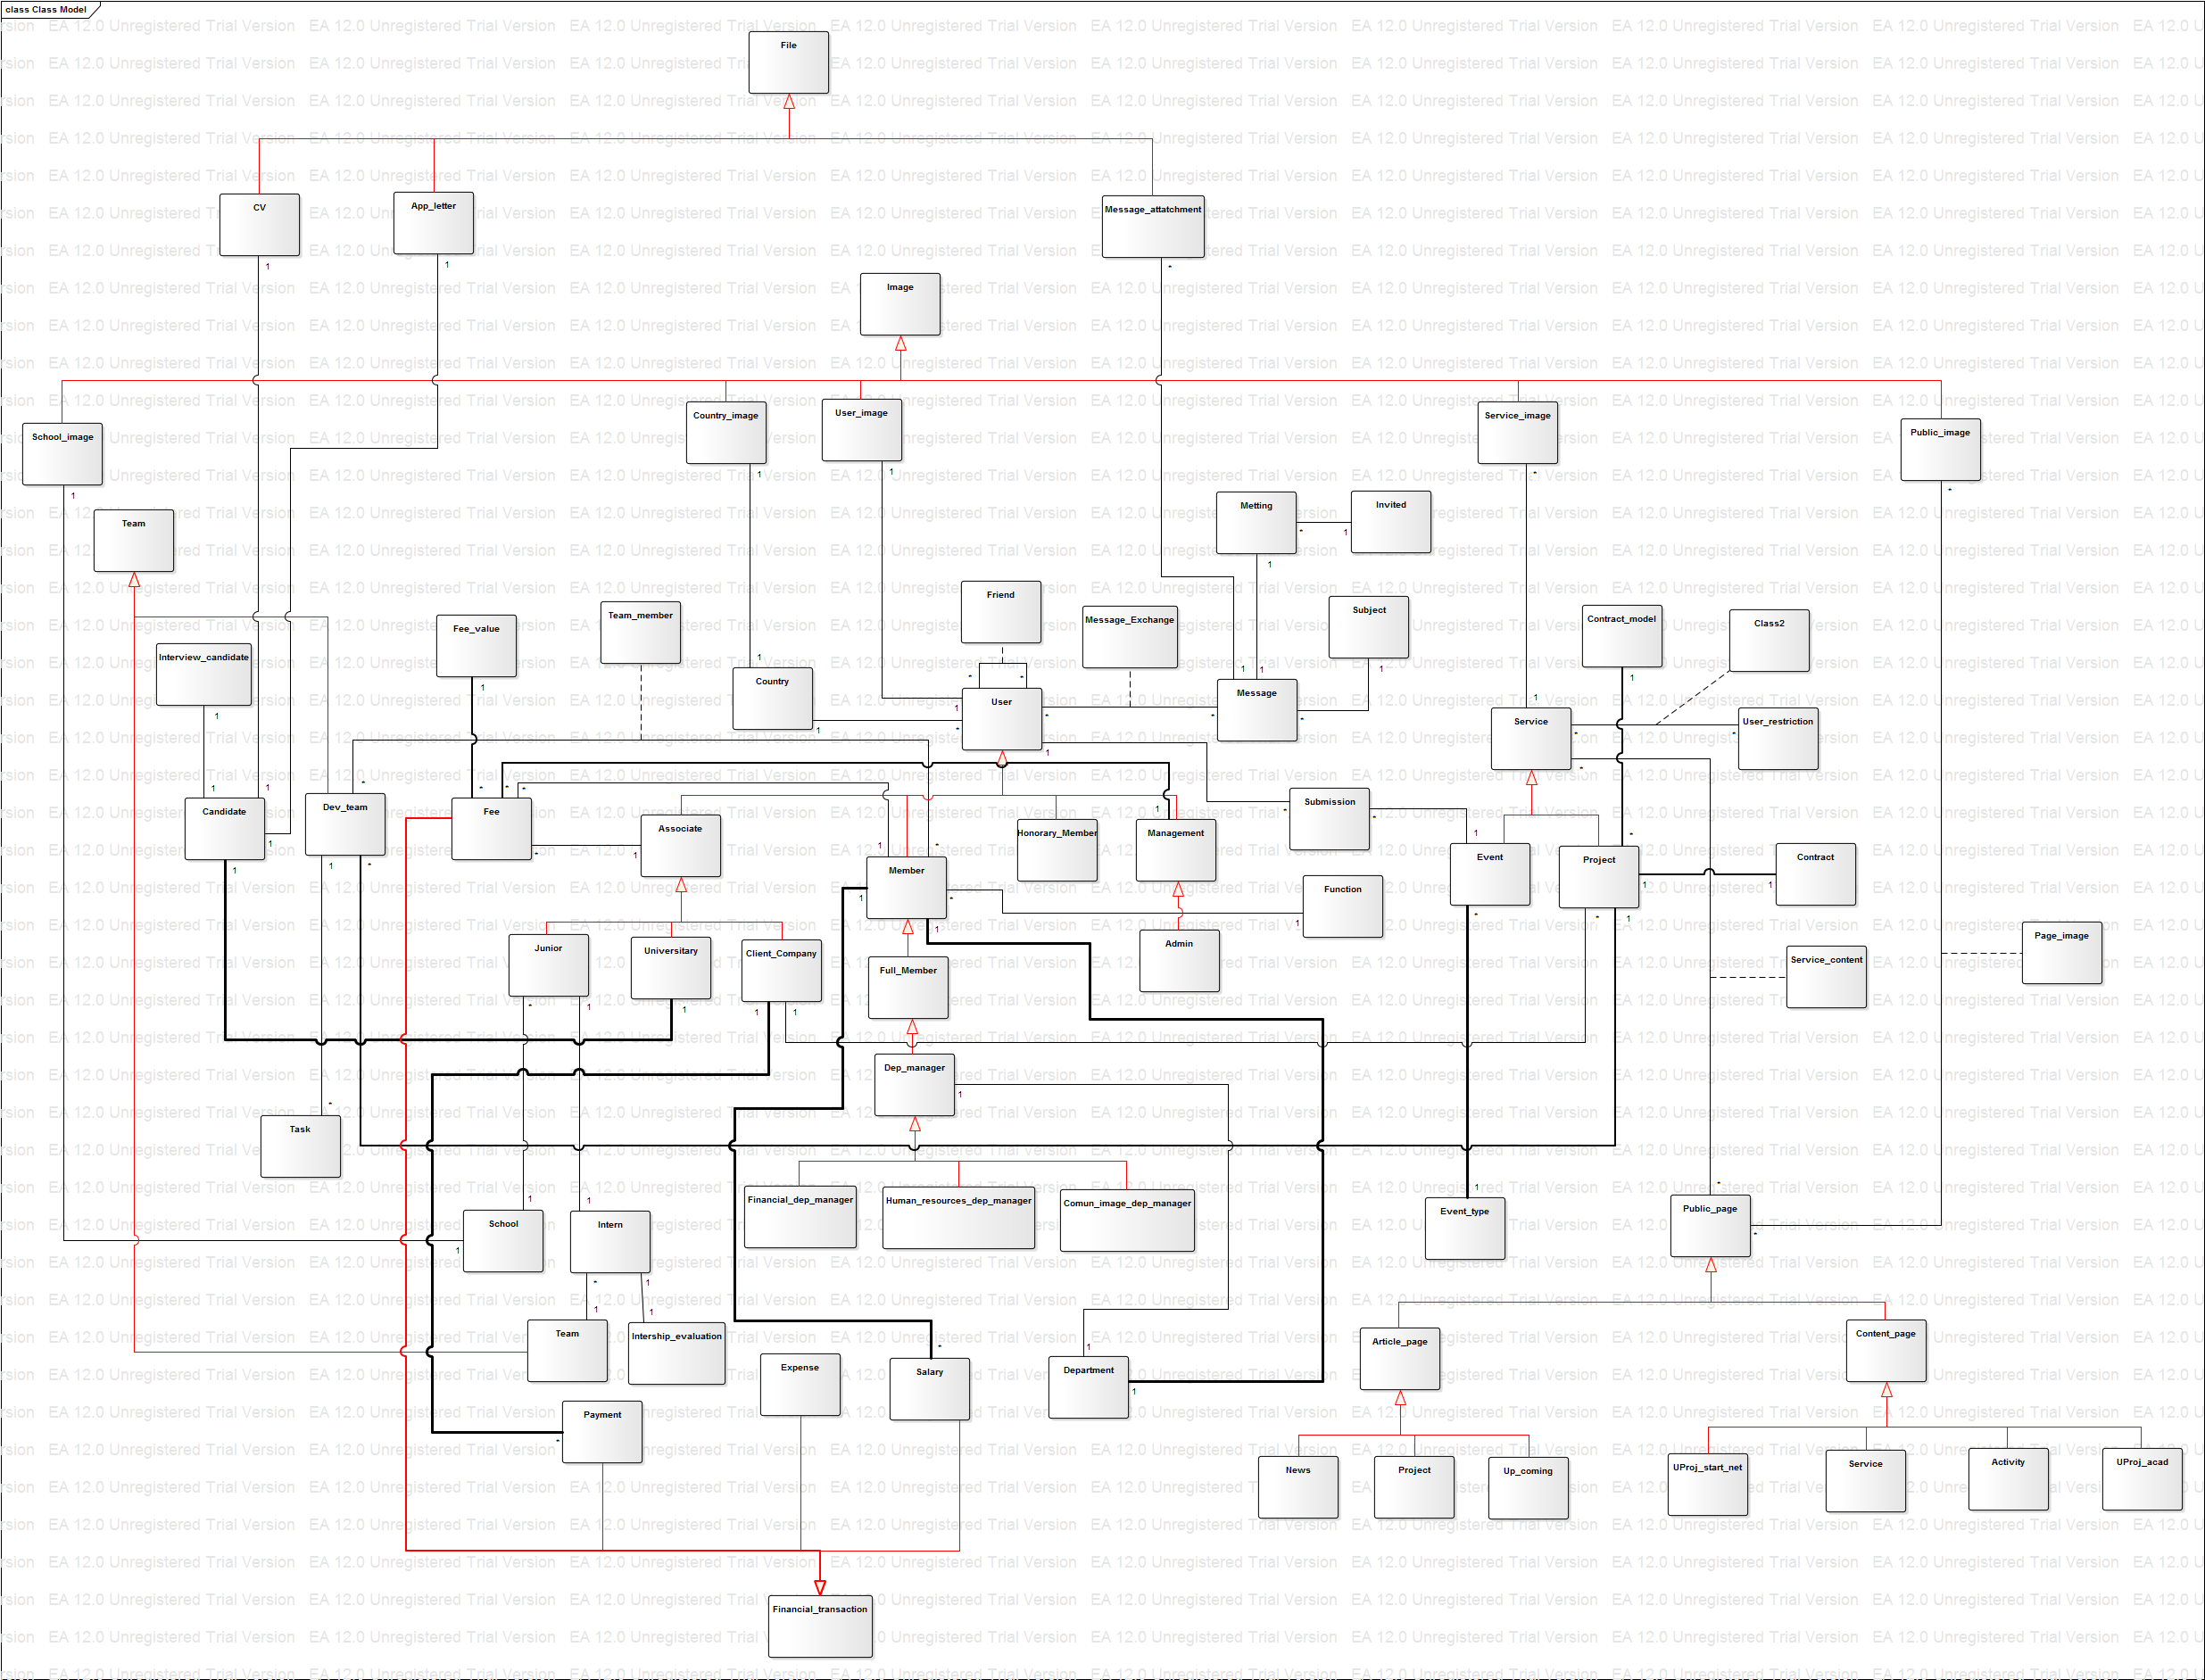
\includegraphics[width=1\linewidth]{Class_Model.png} 
\caption{Figura 29: Modelo UML}

Nesta imagem está representado o modelo UML da base de dados do {\it website}. O modelo UML é uma representação gráfica da estrutura de uma base de dados e serve para mostrar as ligações entre as diferentes tabelas. 
\end{document}